\documentclass[a4paper,12pt,oneside]{book}

% pakiety
\usepackage{polski}
%\usepackage[utf8]{inputenc} % nie można używać as per 
			     % https://tex.stackexchange.com/a/480069/177956
\usepackage{fancyhdr} % nagłówki i stopki
\usepackage{indentfirst} % WAŻNE, MA BYĆ!
\usepackage{graphicx} % to do wstawiania rysunków
\usepackage{amsmath} % to do dodatkowych symboli, przydatne
\usepackage[pdftex,
            left=1in,right=1in,
            top=1in,bottom=1in]{geometry} % marginesy
\usepackage{amssymb} % to też do dodatkowych symboli, też przydatne
\usepackage{pdfpages}
\usepackage{lipsum}
\usepackage{multirow}
\usepackage{listings}
\usepackage{caption}
\usepackage{booktabs}
\usepackage{subcaption}
\usepackage{xcolor}
\usepackage{tikz}
\usetikzlibrary{shapes.geometric, arrows}
\graphicspath{ {./img/} }
\DeclareCaptionType{code}[Listing][Spis listingów] 

\definecolor{codegreen}{rgb}{0,0.6,0}
\definecolor{codegray}{rgb}{0.5,0.5,0.5}
\definecolor{codepurple}{rgb}{0.58,0,0.82}
\definecolor{backcolour}{rgb}{0.95,0.95,0.92}

% tikz shapes for flow diagram
\tikzstyle{terminator} = [rectangle, draw, text centered, rounded corners, minimum height=2em]
\tikzstyle{process} = [rectangle, draw, text centered, minimum height=2em]
\tikzstyle{decision} = [diamond, minimum width=2cm, minimum height=0.5, text centered, draw=black]
\tikzstyle{data}=[trapezium, draw, text centered, trapezium left angle=60, trapezium right angle=120, minimum height=2em]
\tikzstyle{connector} = [draw, -latex']
\tikzstyle{arrow} = [thin,->,>=stealth]


\lstset{
	backgroundcolor=\color{backcolour},   
	commentstyle=\color{codegreen},
	keywordstyle=\color{magenta},
	numberstyle=\tiny\color{codegray},
	stringstyle=\color{codepurple},
	basicstyle=\footnotesize,
	breakatwhitespace=false,         
	breaklines=true,                 
	captionpos=b,                    
	keepspaces=true,                 
	numbers=left,                    
	numbersep=5pt,                  
	showspaces=false,                
	showstringspaces=false,
	showtabs=false,                  
	tabsize=2,
	float=h
}

% definicje nagłówków i stopek
\pagestyle{fancy}
\renewcommand{\chaptermark}[1]{\markboth{#1}{}}
\renewcommand{\sectionmark}[1]{\markright{\thesection\ #1}}
% komenda która sprawi że nie numerowany chapter (chapter*) jest dodany do TOC
\newcommand\chap[1]{%
  \chapter*{#1}%
  \addcontentsline{toc}{chapter}{#1}}
\fancyhf{}
\fancyhead[LE,RO]{\footnotesize\bfseries\thepage}
\fancyhead[LO]{\footnotesize\rightmark}
\fancyhead[RE]{\footnotesize\leftmark}
\renewcommand{\headrulewidth}{0.5pt}
\renewcommand{\footrulewidth}{0pt}
\addtolength{\headheight}{1.5pt}
\fancypagestyle{plain}{\fancyhead{}\cfoot{\footnotesize\thepage}\renewcommand{\headrulewidth}{0pt}}


% interlinia
\linespread{1.25}


% treść
\begin{document}
% strona tytułowa
\sloppy
\thispagestyle{empty}
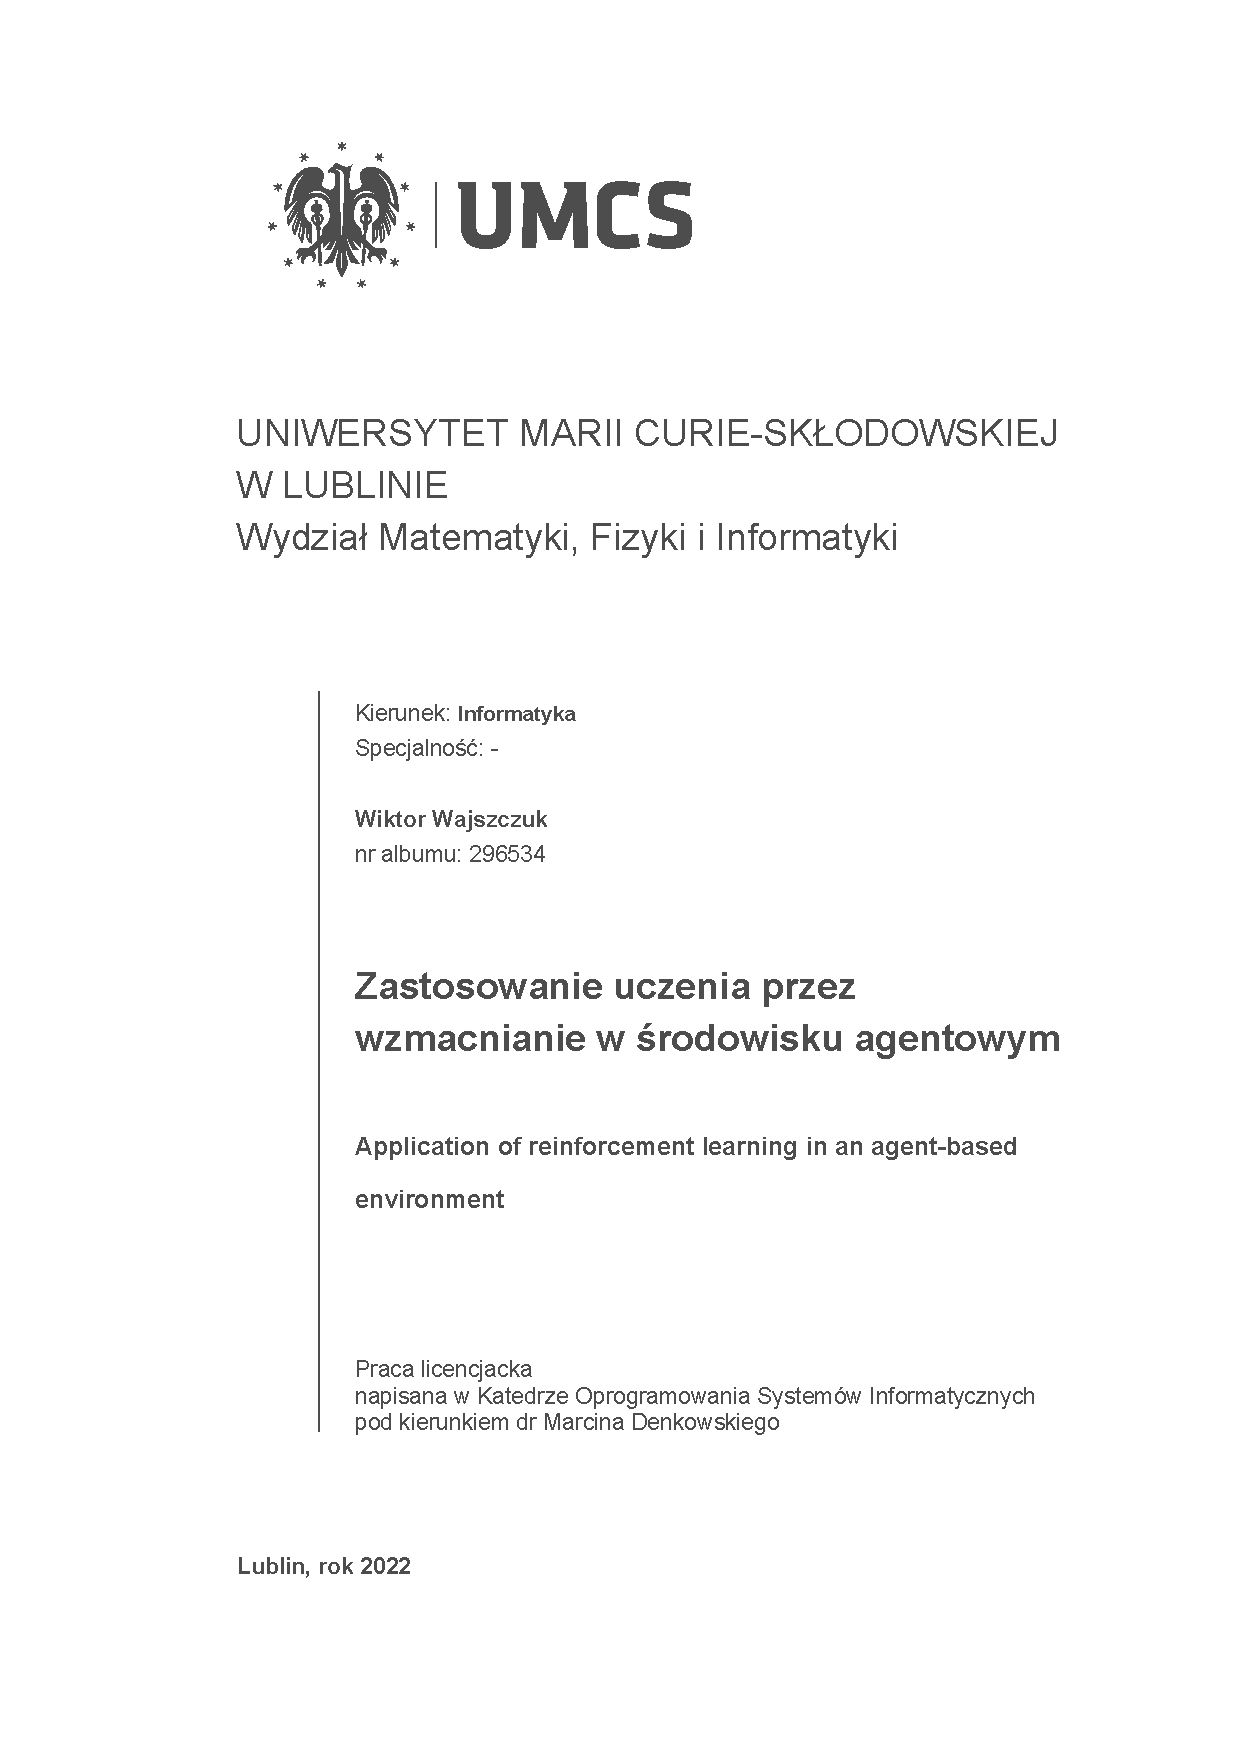
\includepdf{strona_tytulowa}
\newpage{}

\thispagestyle{empty}
\newpage{}

% spis treści
\tableofcontents{}
\newpage

% pusta strona - narazie zakomentowana
%\thispagestyle{empty}
%\
%\newpage

\chap{Wstęp}
Jedną z większych dziedzin uczenia maszynowego jest uczenie przez wzmacnianie (ang.
\textit{reinforcement learning}) W odróżnieniu od zarówno uczenia nadzorowanego i 
nienadzorowanego nie potrzebujemy w tym przypadku żadnych gotowych danych wejściowych i
wyjściowych. Zamiast tego, algorytm pozyskuje dane na bieżąco ze środowiska do, którego
jest zastosowany. Dzięki temu, że algorytmy uczenia przez wzmacnianie nie mają tego
ograniczenia możemy zastosować je do problemów takich jak gra na giełdzie\cite{
trading_reinforcement}, czy nauka grania w gry, w swojej pracy
skupię się na tym drugim.

Celem pracy jest zaimplementowanie algorytmu uczenia przez wzmacnianie \\
Q-Learningu oraz zoptymalizowaniu go tak by po zastosowaniu go do własnoręcznie
zaimplementowanej gry był w stanie osiągnąć w niej możliwie najwyższy wynik.

Na początku przedstawię jaką grę wybrałem, opiszę jej zasady oraz zaprezentuję
szczegóły jej implementacji. Następnie  przybliżę zagadnienie uczenia przez
wzmacnianie oraz algorytmu Q\dywiz learning. Pod koniec pokażę jak
zaimplementowałem wspomniany algorytm, oraz testy po optymalizacjach algorytmu,
które zastosowałem.
\newpage{}

\chapter{Gra}
Problem, który postawiłem przed Q-learningiem to gra z 2013 roku ``Flappy Bird''
autorstwa wietnamskiego developera Dong Nguyena\cite{flappy_bird_author}.
Zdecydowałem się właśnie na tą grę, gdyż sterowanie w niej jest bardzo proste --
jest tylko jeden przycisk do kontrolowania toteż jedna akcja do podjęcia przez
algorytm.
\section{Zasady gry}
\begin{figure}[h]
	\begin{center}
		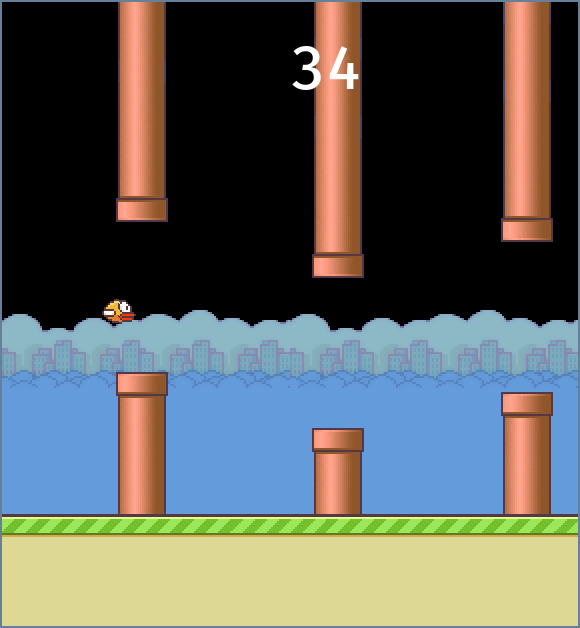
\includegraphics[scale=0.40]{flappy_bird.png}
		\caption{Zrzut ekranu z gry}
		\label{flappy_screenshot}
	\end{center}
\end{figure}

Gracz kontroluje ptaka (na rysunku \ref{flappy_screenshot} kolor żółty),
jego zadaniem jest tak nim sterować by omijać czerwone rury.
Na ptaka działa jedynie siła grawitacji a to rury są przesuwane w jego stronę ze
stałą prędkością. Jak wspomniałem wcześniej gracz ma możliwość jedynie kontrolować
czy ptak załopocze skrzydłami przeciwdziałając sile grawitacji i unosząc się czy
tego nie wykona i opadnie. Gra kończy się gdy ptak spadnie na ziemię 
(część zielona na dole na rysunku \ref{flappy_screenshot}) albo uderzy
w jedną z dwóch nadchodzących do niego czerwonych rur -- dolnej bądź górnej. Punkty
przyznawane są jeżeli graczowi uda się ominąć nadchodzące przeszkody przelatując
przez szczelinę między nimi. Za każde ominięcie przyznawany jest jeden punkt. Jak
widać na rysunku \ref{flappy_screenshot} gracz ominął już trzydzieści par rur.
Podsumowując -- gra sprowadza się do kontrolowania wysokości ptaka tak by ten
przelatywał między nadchodzącymi rurami.

\section{Wykorzystane technologie}
Do zaimplementowania tej gry zdecydowałem się na użycie skryptowego języka
\textbf{python} w wersji 3.8. Wybrałem tą technologię ze względu na prostotę w
pisaniu kodu, świetną dokumentację, fakt, że jest dostępny na większości
współczesnych platform oraz to, że jest to język open\dywiz source.
Dodatkowo wykorzystałem moduł \textbf{pygame}.
\subsection{Pygame}
Pygame dodaje funkcjonalność do biblioteki SDL (więcej o SDLu w następnym podrozdziale).
Pozwala tworzyć w pełni funkcjonalne gry oraz programy multimedialne w pythonie.
Zaletami pygame są między innymi : podstawowe funkcje używają zoptymalizowanego kodu
w C oraz Assembly co sprawia, że pygame jest naprawdę szybkie, podobnie jak python jest
dostępny na większości współczesnych platform oraz prosty w użyciu co zaprezentuję
w części implementacyjnej. Ponadto jest modularny co pozwala programiście używać
tylko tych komponentów, których naprawdę potrzebuje.
\subsection{SDL -- Simple DirectMedia Layer}
Jest to wieloplatformowa biblioteka zapewniająca nisko poziomowy dostęp do audio,
urządzeń peryferyjnych takich jak mysz, klawiatura, joystick, sprzętu graficznego 
(za pomocą OpenGL i Direct3D). Technologia open source zaimplementowana w C.
To za pomocą tej biblioteki pygame może odczytywać wejście czy rysować wyjście 
na ekranie.
\section{Implementacja}
W tym podrozdziale przedstawię w jaki sposób użyłem wyżej wymienionych technologii
do zaimplementowania gry, zacznę od opisania diagramu przepływu.

\begin{center}
\begin{tikzpicture}[node distance = 1.5cm]
\node [terminator] at (0,0) (start) {\textbf{Start}};
\node [process, below of=start] (zainicjalizuj_gre)
{Wczytaj zasoby; zainicjalizuj grę i zegar; zadeklaruj stałe; utwórz grupy};
\node [process, below of=zainicjalizuj_gre] (main_loop) {Main game loop};
\node [decision, below of=main_loop, yshift = -1cm] (900ms) {Minęło 900ms?};
\node [process, right of=900ms, xshift = 3.5cm] (generate_pipes) {Wygeneruj rury};
\node [process, below of=900ms, yshift = -1.7cm] (draw_flappy)
	{Narysuj i zaktualizuj ptaka};
\node [process, below of=draw_flappy] (check_score) {Sprawdź czy przyznać punkt};
\node [decision, below of=check_score, yshift = -0.5cm] (check_collision)
	{Kolizja?};
\node [data, below of=check_collision, yshift = -0.9cm] (check_input) {Sprawdź input};
\node [decision, below of=check_input, yshift = -0.5cm] (check_esc) {ESC?};
\node [decision, below of=check_esc, yshift = -0.9cm] (check_lpm) {LPM?};
\node [process, right of=check_lpm, xshift = 2.5cm] (flap) {Pomachaj skrzydłami};
\node [process, below of=check_lpm, yshift = -0.8cm] (display_update)
	{Zaktualizuj ekran};
\node [terminator, below of=display_update] (end_game) {\textbf{Koniec gry}};
\draw [arrow] (start) -- (zainicjalizuj_gre);
\draw [arrow] (zainicjalizuj_gre) -- (main_loop);
\draw [arrow] (main_loop) -- (900ms);
\draw [arrow] (900ms) -- node[anchor=east] {Nie} (draw_flappy);
\draw [arrow] (draw_flappy) -- (check_score);
\draw [arrow] (check_score) -- (check_collision);
\draw [arrow] (check_collision) -- node[anchor=east] {Nie} (check_input);
\draw [arrow] (check_input) -- (check_esc);
\draw [arrow] (check_esc) -- node[anchor=east] {Nie} (check_lpm);
\draw [arrow] (check_lpm) -- node[anchor=east] {Nie} (display_update);
\draw [arrow] (display_update) -- (end_game);
\draw [arrow] (900ms) -- node[anchor=south] {Tak} (generate_pipes);
\draw [arrow] (check_lpm) -- node[anchor=south] {Tak} (flap);
\draw [arrow] (generate_pipes) |- (draw_flappy);
\draw [arrow] (flap) |- (display_update);
\node [right of = check_collision, xshift = 5cm, inner sep=0pt, outer sep=0pt]
	(phantom_collision) {};
\draw [arrow] (check_collision) -- (phantom_collision);
\node [right of = check_esc, xshift = 5cm, inner sep=0pt, outer sep=0pt]
	(phantom_esc) {};
\draw [arrow] (phantom_collision) -- (phantom_esc);
\draw [arrow] (check_esc) -- (phantom_esc);
\draw [arrow] (phantom_esc) |- (end_game);
\node [left of = display_update, xshift = -3cm, inner sep=0pt, outer sep=0pt]
	(phantom_display_update) {};
\draw [arrow] (display_update) -- (phantom_display_update);
\draw [arrow] (phantom_display_update) |- (main_loop);
\end{tikzpicture}
\end{center}
\newpage{}
Tutaj będą opisane po kolei nody co robią na diagramie

\chapter{Uczenie przez wzmacnianie}
Tutaj do napisania o tym czym jest uczenie przez wzmacnianie pare slow jakie są algorytmy
jak działa, schemat środowisko - agent - akcja - reward
\section{Q\dywiz learning}
Tutaj wszystko związane z qlearningiem, wzory, itp :)

\chapter{Implementacja Q\dywiz learningu}
Tutaj fragmenty kodu, jakie zmiany dokonałem względem książkowego algorytmu
\section{Podejście pierwsze grid 10 na 10}
Po kolei wyjaśnienie co to grid 10 na 10 jak to jest implementowane itp
\section{Podejście drugie grid 10 na 10 i flaga za śmierć od wysokiej rury}
Jak wyżej
\section{Podejście trzecie grid 5 na 5 z flagą}
Jak wyżej

\chapter{Podsumowanie}
Wyniki osiągane są w miarę ok ale mogło by być lepiej bo są na internecie lepsze
podejścia do tego problemu -- być może wynika to z tego ze sam implementowałem grę
i nie jest ona tak dobrze przetestowana jak ta dostępna na GitHub?
\section{Co można by ulepszyć}
Tutaj będę pisał co mogłem zrobić gdybym poświęcił więcej czasu np:
\begin{itemize}
\item uczenie bez wizualizacji pygamowej
\item zrównoleglenie by paru agentów na raz mogło się uczyć
\item doszlifowanie algorytmu??
\end{itemize}


\addcontentsline{toc}{chapter}{Bibliografia}
\bibliographystyle{IEEEtran}
\bibliography{praca_licencjacka}

\end{document}
